\documentclass{article}
\usepackage[utf8]{inputenc}
\usepackage{subcaption}
\usepackage{amsmath}
\usepackage{amssymb}
\usepackage{hyperref}
\usepackage{titlesec}
\usepackage{xcolor}
\usepackage{fancyhdr}
\usepackage{graphicx}
\usepackage{multirow}
\usepackage[rightcaption]{sidecap}
\usepackage{verbatim}
\usepackage[backend=bibtex]{biblatex}
\usepackage [ a4paper , hmargin =1.2 in , bottom =1.5 in ] { geometry }
\hypersetup{
    colorlinks=true,
    linkcolor=blue,
    filecolor=magenta,      
    urlcolor=cyan,
}

% Add header and footer code here
\fancyhf{}
\fancyfoot[C]{Page \thepage}
\lhead{Transformation of R.V. and Multivariate Gaussian}
\rhead{Aditya Neeraje}

\title{Transformation of R.V. \\ and \\ Multivariate Gaussian}
\author{Aditya Neeraje}
\date{}

% You may also add path to the images optionally
\bibliography{references}
\graphicspath{ {./images/} }

\begin{document}
\pagestyle{fancy}
\maketitle

% preamble

% below line auto generates the table of contents
% thank me for your free 1 mark
\tableofcontents
\clearpage

%code of section 1, with lists
\section{Introduction}
In this article, we will study about the following topics of statistics:
\begin{itemize}
    \item Transformation of random variables
    \item Multivariate Gaussian random variables
\end{itemize}

%code of section 2, make appr
\section{Transformation of Random Variable}
Given any continuous r.v $X$ with PDF $P_{X}(x)$ and given any function $g(X)$ (defined on range of $X$) we intend to find PDF associated with the r.v $Y = g(x)$.\\
For simplicity, let's assume $g(.)$ is monotonic increasing.\\
Then by probability mass conservation,
\[
    P(a < X < b) = P(g(a) < Y < g(b)) = \int_{g(a)}^{g(b)}Q(y) \,dx\
\]
Using $y=g(x)$, we get the below relation upon simplification
\[
    Q(y) = P(y^{-1}(y))\frac{d(g^{-1}(y)}{dy}
\]
To handle monotonically decreasing $g(.)$ as well
\footnote{\label{foot:ref_1}we could have used modulus operator but I wanted things to look more complicated}

\begin{equation}
    Q(y) = 
    \begin{cases}
        +P(y^{-1}(y))\frac{d(g^{-1}(y)}{dy} & \text{for } g(.) \text{ monotonically increasing}\\
        -P(y^{-1}(y))\frac{d(g^{-1}(y)}{dy} & \text{for } g(.) \text{ monotonically decreasing}\\
    \end{cases}
\end{equation}
For more information, refer \cite{url:transformations}

\begin{figure}[h!]
     \centering
     \begin{subfigure}{0.49\textwidth}
         \centering
         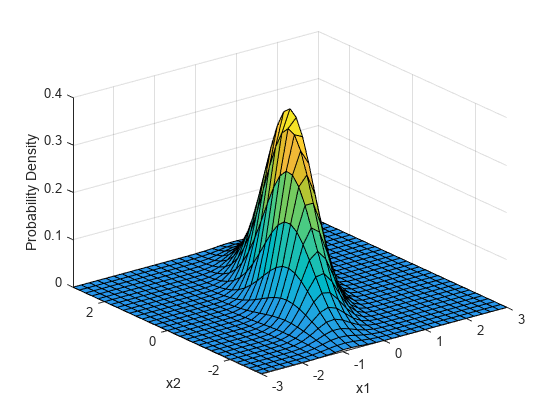
\includegraphics[width=\textwidth]{multivariate_gaussian}
         \caption{Example 1}
         \label{fig:ex_1}
     \end{subfigure}
     \hfill
     \begin{subfigure}{0.49\textwidth}
         \centering
         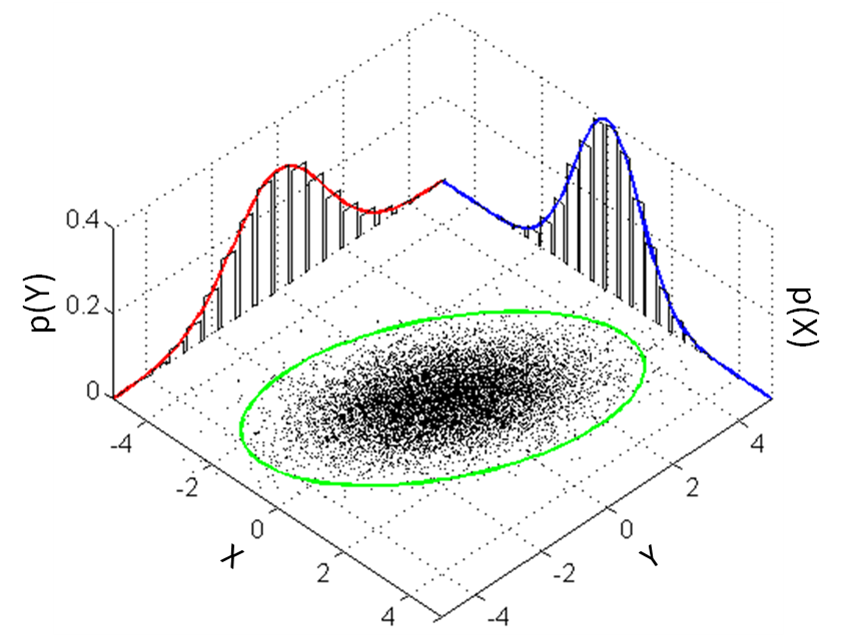
\includegraphics[width=\textwidth]{multivariate_normal}
         \caption{Example 2}
         \label{fig:ex_2}
     \end{subfigure}
     \hfill
\end{figure}

%code for section 3
\section{Multi-variate Gaussian Distribution}
\subsection{Definition}
Let $X$ be a vector of random variables of Dimension $D$.\\
A r.v. $X$ has a joint PDF as multi-variate Gaussian distribution $\exists$ finite i.i.d. standard Gaussian r.v. $W_1, W_2,\dots,W_N$ with $N > D$ such that\\
\[
    X = AW + \mu
\]
Refer fig[\ref{fig:ex_1}] and fig[\ref{fig:ex_2}] for visual examples. This has many applications in machine learning, refer \cite{book:carl_edward} and \cite{url:gaussian_processes}.

\subsection{A is diagonal}
In this case, the $X_i$ are independent. The standard deviation of distribution of $X_i$ is $A_{ii}$.

\subsection{A is non-singular square matrix}
Let's take $\mu = 0$ for simplicity.\\
Similar to the univariate case, where scaling was determined by $\left|\frac{d(g^{-1}(y))}{dy}\right|$, the scaling for multi-variate case is determined by determinant of matrix of derivatives, Jacobian matrix.
Also, $W=A^{-1}X$, which is a linear transformation of vector $X$. $A^{-1}$ maps a hypercube to a parallelopiped. If the vectors describing the hypercube are along the cardinal axis, then the parallelopiped is described by vectors which are columns of $A^{-1}$.\\
We intend to find the volume of the parallelopiped formed due to this transformation.\\
\textbf{Claim: }The volume of parallelopiped described by column vectors of matrix $A^{-1}$ is given by $det({A^{-1}})$\\
\textbf{Proof: }Addition of any scaled column of a matrix $M$ to another column does not change the determinant.\\
Therefore by Gram-Schmidt orthogonalization process the columns of $A^{-1}$ can be constructed to be orthogonal to each other, without changing the determinant. Then multiplying by an orthogonal matrix would rotate the orthogonal vectors(to align them with cardinal axis), and this operation would not change the determinant as well. Now the result matrix is diagonal square matrix and the volume of the parallelepiped described by the column vectors is given by product of diagonal elements.\\
\\
From the above result, an infinitesimal volume $\delta^{D}$ after transformation becomes $\delta^{D} \cdot det(A^{-1})$.\\
\\
Let $C=A \cdot A^T$. Then $det(A) = \sqrt{det(C)}$. The above expression can be rewritten as
\begin{equation}
    P(X) = \frac{1}{(2\pi)^{D/2}}\cdot \frac{1}{\sqrt{det(C)}} \cdot exp(0.5 \cdot X^T \cdot C^{-1} \cdot X)
\end{equation}
\begin{tabular}{|c|c||c|}
\hline
\multicolumn{3}{|c|}{Sample Values of bivariate normal distribution}\\
\hline
x & y & f(x,y)\\
\hline
 0 & 0   &  1.6\\
0   &  1 & 0.096 \\
$\sqrt{2}$ & $\sqrt{2}$ & 0.02 \\
\hline
\end{tabular}

% print the bibliography
\printbibliography

\end{document}
